\documentclass[../../main.tex]{subfiles}

\graphicspath{{images/Fahrdaten/}{../../images/Fahrdaten/}}

\begin{document}
\subsubsection{Beschleunigung}
Mithilfe elektronischer Komponente kann Beschleunigung, Geschwindigkeit und Distanz(vom Startbereich) gemessen und analyiert werden. Zusätzlich kann eine approximierte Position des Zuges auf der Strecke berechnet werden.

\paragraph{Anforderungen}
\begin{itemize}
    \item Momentane Beschleunigung auslesen
    \item Beschleunigung in Geschwindigkeit und Distanz umrechnen
    \item Approximierte Position berechnen (wo auf der Strecke befinden wir uns)
    \item Auf wenige cm genau anhalten
    \item (Optional) Zentrifugalkräfte in Kurven berechnen
\end{itemize}

\paragraph{Konzept}
Über ein Beschleunigungssensor werden Beschleunigung und Rotation ausgelesen. Die Beschleunigung kann zusätzlich in Geschwindigkeit und Distanz umgerechnet werden.

\paragraph{Komponente}
Bei der Komponentenwahl haben wir uns für einen Adafruit i2c 3-Achsen Beschleunigungssensor entschieden, dieser kann Beschleunigung sowie Rotation berechnen. Er weist eine sehr kompakte Bauform auf und ist relativ günstig zu erwerben. Online haben verschiedene Nutzer mit dieser Komponente positive Erfahrung gesammelt. Auch ist die Komponente gut dokumentiert und man findet verschiedene Tutorien wie man diese mit einem Raspberry Pi kombinieren kann.

\begin{table}[] \centering
\begin{tabular}{lll}
Name & Adafruit ADXL 345 \\
Preis & 1Fr    \\
Länge & 25mm    \\
Breite & 19mm   \\
Höhe & 3.14mm      \\
Gewicht & 1.27g   \\
Leistung & 3V \\
\end{tabular}
\end{table}

\subparagraph{Bauplan / Interface}
\begin{figure}[H] \centering
  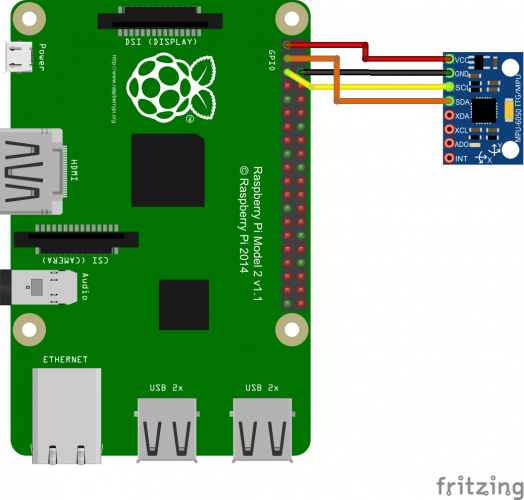
\includegraphics{Verkabelung_BeschlSensor}
  \caption{Verkabelung Beschleunigungssensor}
  \label{fig:Beschleunigungssensor}
\end{figure}

\begin{table}[] \centering
\begin{tabular}{lll}
Bezeichnung     & GPIO Bus & MPU 6050 \\
Stromversorgung & 3V3      & VCC      \\
Ground          & GND      & GND      \\
Daten          & SDA      & SDA      \\
Clock          & SCL      & SCL
\end{tabular}
\end{table}

Der Sensor wird über die i2c Schnittstelle angesprochen und verwendet somit einen Datenport (SDA) und eine Clock (SCL). Für die Stromversorgung reicht der 3.3V Port (3V3) und der Ground (GND) des GPIO Buses.

\subparagraph{Daten}
Mithilfe eines Skripts erhalten wir eine gute übersicht der erhaltenen Daten.

\begin{lstlisting}
Gyroskop

gyroskop\_xout:   -260  skaliert:  -2
gyroskop\_yout:   -154  skaliert:  -2
gyroskop\_zout:     78  skaliert:  0

Beschleunigungssensor

beschleunigung\_xout:   -1048  skaliert:  -0.06396484375
beschleunigung\_yout:    -676  skaliert:  -0.041259765625
beschleunigung\_zout:   16644  skaliert:  1.01586914062
X Rotation:  -2.32121150537
Y Rotation:  3.59994842011
\end{lstlisting}

\paragraph{Realisierung}








\end{document}
